\documentclass[oneside]{book}

	%FORMATTING
	 	\usepackage{graphicx} %op shit
	 	\usepackage[margin=1in]{geometry} %Set margins
	 	\usepackage{fixltx2e} %subscript
	 	\usepackage{multicol} % multiple columns
	 	\usepackage[toc]{appendix} % Allows appendices
	 	\usepackage{float}
	 	\usepackage{textcomp}
	 	\usepackage{CJKutf8} %japanese support
	 	\usepackage{hyperref} % urls, chapter ref
	 	\usepackage{footnote}
	 	\usepackage{makecell}
	 		\makesavenoteenv{tabular}
	%LINGUISTICS-RELATED PACKAGES
	 	\usepackage{qtree} %syntax trees
	 	\usepackage{covington} %interlinearizations
	 	\usepackage{amsmath,amsthm,amssymb} %empty set and some other shit
	 	\usepackage{tipa} %ipa
	 	\usepackage{vowel}

	 \let\oldemptyset\emptyset %Redefines the shitty empty set symbol to the old one.
	 \let\emptyset\varnothing

	 \newcommand{\entry}[4]{\markboth{}{}\textbf{#1}\ {[#2]}\ \textit{#3}\ $\diamond$\ {#4}}  % dictionary command

	 \newcommand{\uline}{\rule[-5pt]{20pt}{1pt}} % line for phon rules

	 %stuff for handling how awful it is to use default tipa syntax
	 	\newcommand{\R}{\textipa{R}} %alv tap
	 	\newcommand{\N}{\textipa{N}} %eng
	 	\newcommand{\OO}{\textipa{O}} %open o, DONT FORGET THE SECOND O!!!
	 	\newcommand{\B}{\textipa{B}} %bilab fric voi
	 	\newcommand{\G}{\textipa{G}} %velar fric voi
	 	\newcommand{\W}{\textipa{V}} %bilab approximant
	 	\newcommand{\F}{\textipa{F}} %-voi bilab fric
	 	\newcommand{\M}{\textturnmrleg} %velar approx
	 	\newcommand{\glot}{\textipa{P}}
	 	\newcommand{\len}{\textipa{:}} % long vowels and shit

		\newcommand{\tie}[2]{\textipa{\t{#1#2}}} % tie bars

	 	\newcommand{\0}{$\emptyset$} %Null
	 	\newcommand{\D}{\scshape} %smallcaps
	 	\newcommand{\stress}{\textquotesingle}

	 	\newcommand{\kurango}{K\textipa{uRaNO}}
	 	\newcommand{\nom}{\D{nom}}
	 	\newcommand{\erg}{\D{erg}}
	 	\newcommand{\abs}{\D{abs}}
	 	\newcommand{\gen}{\D{gen}}
	 	\newcommand{\poss}{\D{poss}}
	 	\newcommand{\emo}{\D{emo}}
	 	\newcommand{\cop}{\D{cop}}
	 	\newcommand{\caus}{\D{caus}}
	 	\newcommand{\pst}{\D{pst}}
	 	\newcommand{\fut}{\D{fut}}
	 	\newcommand{\negative}{\D{neg}}
	 	\newcommand{\interr}{\D{interr}}
	 	\newcommand{\reas}{\D{reas}}
	 	\newcommand{\dirprox}{\D{dir:prox}}
	 	\newcommand{\pl}{\D{pl}}
	 	\newcommand{\redupl}{\D{redup.pl}}

	 	\newcommand{\tild}{{\raise.17ex\hbox{$\scriptstyle\sim$}}} % tilde

	% Commands for dealing with custom fonts
	% http://math.stanford.edu/~jyzhao/latexfonts.php
	% http://xpt.sourceforge.net/techdocs/language/latex/latex33-LaTeXAndTrueTypeFont/ar01s03.html
		\newcommand\customfont[1]{{\usefont{T1}{custom}{m}{n} #1 }}

%--------------------------------------------------------------%
%  EXAMPLE INTERLINEAR GLOSS, ADAPTED FROM LEV'S DISSERTATION  
%															   
%	\begin{example}											   
%	\label{ex:nasalpoa}										   
%		Ontagake. \textipa{[ontagakse]}						   
%		\gll o= n- tag -ak -e 								   
%		3nmS= irreal burn -perf -irreal.i 					   
%		\glt `It will burn.' 								   
%		\glend 												   
%	\end{example} 											   
%  															   
%	%Reference examples like this: (\ref{ex:nasalpoa})         
%--------------------------------------------------------------%

\begin{document}

	\begin{titlepage}
\centering
	{\huge\bfseries \kurango \par}
	\begin{center}
	{
\includegraphics[scale=0.3]{./img/kurango.png}}
	\end{center}
		\vspace{2cm}
	{\Large\itshape Garret Kurteff\par}
		\vfill
	{\large \today\par}
\end{titlepage} % Title page
	\section*{To-do}

\emph{This section will be omitted in the final compile. It's so Garret knows what to work on.}\\

Sections to write from notebook:
	\begin{enumerate}
		\item Lexically different types of intelligence.
		% Kura -tifi = something good as an easter egg
		\item case assignment
		\item add \emph{rha} as itself for a noun that means thought. Makes a lot more sense for your compounding ideas that you were meditating upon.
	\end{enumerate}

The -ti/opposite edge reduplication issue is pretty pressing. for the sake of continuity i prefer to use OER but the nana/nini/nunu thing might be too salient to use that. think of some historically motivated solution? the current one is kind of weak.

Old stuff to consolidate:
	\begin{enumerate}
		\item check interlins
		\\ Maybe like print out a copy and make sure everything is up to date (physical proofreading ftw)(for the interlins only.)
		\item move unfinished ``philosophy'' section to the introduction instead?
			\\ finish it too lol
	\end{enumerate}

New stuff to write:
	\begin{enumerate}
		\item Think of a system of encoding grammatical mood. This is necessary in order to complete your own litmus test, a translation of the ``Litany Against Fear.'' Moods that already have a gloss: Indicative(\0), Imperative(\R\OO), Interrogative(\R i); Moods that need a gloss: Conditional ``would'', Subjunctive ``if'', Potential ``may''
		\item Think of ways to incorporate zero-derivation that won't fuck with the use of your causative. Trigger: salience, close semantic proximity, etc. (god forbid something is COMPLETELY irregular)
		\item Culture/sociolinguistics/dialectology section? (Talk about the progressive--descriptive vs conservative--prescriptive dialects.)
		\item WH QUESTIONS!!! look at discussion with jenks. u need a new lexical entry for this.
		\item Where are you going to put your morphosyntax section? (A: probably in with the morphology as you introduce concepts.)
		\item section on adverbial constructions
		\item Different morphological topics
		\\ Like, prox/dist/near/far distinction (Should probably go in case section)
		\item Inflectional morphology (how 2 organize?)
		\item Derivational morphology (how 2 organize?)
		\\ 1 section on the dedicated class changers
		\\ 1 section on everything else? % Do you even need these sections?
		\item word order section (under grammar)
		\item a ``fun facts'' appendix or some shit?? maybe put in intro instead?
		\item Suprasegmental stuff. (tone, stress, others)
		\item Some phonology about vowel deletion in common grammatical forms (person markers, tense markers, etc) to form nasal consonant clusters? u need those nasals bb
		\item eventually find some way to make numeracy not as lame.
	\end{enumerate}

Stuff to yoink from the wiki:
	\begin{enumerate}
		\item person marking/(Case too?) (put in DP section under Constituency in Grammar)
		\item Mass (next to numeracy in morpho) % Move both of these to QP?
		\item Greetings (the appendix?)
		\item Enclitics (is this even relevant anymore? in the grammar section?)
	\end{enumerate}

\clearpage % TO DO, DELETE THIS
	\section*{Notes/Acknowledgements}

Left blank for now.

% vlad for testing
% dad for debate about emotions
% inkelas/holland
% karen / DJP / quijada for inspiration
% lev for helping me with some typo stuff

\section*{Philosophy/Design Goals}

Many conlangers try to tailor their languages to their languages' respective cultures (Dothraki), or create languages as thought experiments (Ithkuil). Because I am both an academically-trained linguist and an amateur conlanger, I did neither.

% typologically optimal
% lang for linguists

% DESIGN GOALS
	% no portmanteau morphemes
	% Permutable phonetic system
	% No redundancy
	% VPiSH
	% Permutable orthography
	% Emotion expression
% Maybe move design goals to beginning of each chapter?
	% yeah do this............ but also mention in the intro or osme shit?
	% DO you even need an intro?

 % acknowledgements/etc

	\setcounter{tocdepth}{1}
	\tableofcontents

	\chapter{Introduction}

``To be honest, a large part of [whether or not I was working on Ithkuil] was dependent on whether or not I was in a relationship at the time.'' -- John Quijada % introduction
	\chapter{Syntax}
	
	\section{Word order} 
		{\kurango} has a fixed SVO word order. The case assignment system is what makes the word order fixed (see Section \ref{case}).
		\subsection{Constituent order} % head final
		\subsection{Placement of adjuncts}
		% Consituent order (head final)
		% Also word order (SVO)
	\section{Morphological type} % Explain why you are putting this under syntax, include the figure from C+B, explain dialectical differences between this (conservative should be more isolating, more polysynthetic)

	\section{Case system} % accusative vs ergative
	\label{case}
		In \kurango , basic subject/object case assignment is based on word order. Arguments to left of the verb get ergative case, and arguments to the right of the verb get absolutive case. For {\D{erg}} and {\D{abs}}, there are no explicit case markers.



		\begin{example}
		\label{ex:case_wordorder_1}
			Ni'inakarana. [\textipa{niPinakaRana}]
			\gll ni- inakara -na
			2- bore -1
			\glt `You bore me.'
			\glend
		\end{example}

		\begin{example}
		\label{ex:case_wordorder_2}
			Na'inakarani. [\textipa{naPinakaRani}]
			\gll na- inakara -ni
			1- bore -2
			\glt `I bore you.'
			\glend
		\end{example}

		This ordering principle also allows us to categorize {\kurango} as a Fluid-S language, as arguments of intransitive verbs (S) pattern either with subjects of transitive verbs (S\textsubscript{A}) or objects of transitive verbs (S\textsubscript{O}) based on their position relative to the verb. Determining the way in which S patterns has to do with the semantics of the utterance: S\textsubscript{A} (marked with {\D{erg}}) has no entailment about the volition of the Agent in the action being performed, while S\textsubscript{O} (marked with {\D{abs}}) entails that the agent was volitional in the action being performed.

		\begin{example}
		\label{ex:case_erg}
			Nakari. [naka\R i]
			\gll na- kari
			1- sleep
			\glt `I sleep.' (by my own volition.)
			\glend
		\end{example}

		\begin{example}
		\label{ex:case_abs}
			Karina. [ka\R ina]
			\gll kari -na
			sleep -1
			\glt `I sleep.' (no entailment about my volition.)
			\glend
		\end{example}
	% Technically it's SVO, but, mention how it can be SV or VS in intransitive sentences (fluid S system)
		\subsection{Auxillary cases}
			In addition to the basic cases assigned by syntactic position, there are additional cases assigned by explicitly marked D- or P-heads. Below is a list and examples:
				\subsubsection{Genitive}
					Genitive (posessive) case is assigned by a postponed determiner \emph{-mi}.
					% example
				\subsubsection{Inessive}
					make a gloss for this
					% ``in the house''
				\subsubsection{Elative}
					% out of the house
				\subsubsection{Illative}
					% into the house
				\subsubsection{Adessive}
					% To the house
				\subsubsection{Ablative}
					% away from the house
				\subsubsection{Allative}
					% to the house

% Kurango:
	% Word order: SVO
	% No movement(adheres to VPiSH)
	% Head-final
	% Agglutinating with mild polysynthesis
	% Fluid S system

% Questions for Jenks:
	% Draw these trees:
		% Deep structure of English "He sees me"
		% Deep structure of English "The cat will give the mouse a scare"
		% Deep structure of an English yes/no question
		% Deep structure of an English wh-question
		% Deep structure of an English intransitive sentence
		% Deep structure of Negated english sentences
		% Deep structure of 'do' support
		% Deep structure of multi-clausal english sentences
		% The VPiSH sentence
	% Examples of languages without movement << Mandarin? Is there such a language?
	% Can a language be head-initial AND head-final based on different contextual rules?


% Head final under head initial (Think of german.)


% Subject: spec lil vp
% Object: spec VP

% Right branching = head on left

% Dative argument: Comp V


% DEEP STRUCTURE
	
 % syntax chapter
	\chapter{Phonetics}
\label{chap:phone}

\kurango, being an academically-minded language, has an unnatural, engineered phonology tailored for its orthographic system\footnote{For more on the orthography, please refer to \autoref{chap:ortho}.}. However, there is some allophony, not to sell the phonetic system as entirely robotic.

\section{Consonants}
In short, there are three kinds of contrasts in \kurango: voicing, place, and manner. Permutably, there are three places of articulation, four manners of articulation, and two voicing methods. This allows for the existence of 24 phonemes, but, due to typological rarity, voiceless nasals and approximants have been omitted. There is also a glottal stop /\glot/ because glottal stops are awesome.

	\begin{figure}[H]
	\label{permute_cons}
	\begin{enumerate}
	\centering
		\item[Manner:] [+nasal], [-cont, -son], [+cont, -son], [+cont, +son]
		\item[Place:] [+labial], [+coronal], [-coronal]
		\item[Voice:] [+voice], [-voice]
	\end{enumerate}

	\begin{center}
		\caption{Possible values for permutable categories in {\kurango} consonants}
	\end{center}
	\end{figure}

The below consonant chart may help indicate my point. Items in parentheses are used only in allmorphy, items joined with tildes are in free variation.
	
	\begin{table}[H]
	\centering
	\caption{Consonant chart for \kurango}
	\label{conschart}
		\begin{tabular}{ccccc}
		 & Labial & Alveolar & Velar & Glottal \\ \hline\hline
		Nasal & m & n & \N & \\ \hline
		Stop & p b & t d & k g & \glot \\ \hline
		Fricative & {\F} \B & s z & x \G & \\ \hline
		Sonorant & {\W} (w) & \R\tild\textipa{\*r}\tild r &{\M} (j\footnotemark) & \\ \hline\hline
		\end{tabular}
	\end{table}
	\footnotetext{Yes, I know /j/ is palatal, fuck you}

For information on allophony, see \autoref{chap:phono}.

\section{Vowels}
\kurango's vowel system is also ``engineered'' based off permutable contrasts, with height and laterality being contrastive. Roundness is non-contrastive, but front\footnote{Technically, non-back vowels as /a/ is [-front, -back].} vowels are [-round] and back vowels are [+round]. Vowels also contrast in length.

	\begin{figure}[H]
	\label{permute_vow}
	\begin{enumerate}
	\centering
		\item[Height:] [+high], [-high]
		\item[Laterality:] [+back], [-back]
	\end{enumerate}

	\begin{center}
		\caption{Possible values for permutable categories in {\kurango} vowels}
	\end{center}
	\end{figure}

Also, a vowel trapezium:

	\begin{figure}[H]
	\label{trapezium}
	\begin{center}
		\begin{vowel}[three]
			\putcvowel[l]{i}{1}
			\putcvowel[l]{a}{4}
			\putcvowel[r]{u}{8}
			\putcvowel[r]{\textopeno\tild o}{6}
		\end{vowel}
	\caption{Vowel trapezium for \kurango}
	\end{center}
	\end{figure}

There isn't much else to say about vowels, except that /\OO/ is often phonetically lower than it appears in standard IPA, making it sound closer to [\textipa{6}]. L1 bias may cause some {\kurango} vowels to phonetically shift: for me (a Californian), /\OO/ is closer to [o], /u/ is closer to [\textipa{1}], and /a/ is centralized. % phonetics
	\chapter{Phonology}
\label{chap:phono}

\section{Allophony}

Because \kurango's phonetic inventory is based around the idea of permutation, there is very little allophony. Most allophony in the language is the result of ameliorating coarticulatory strain.

	\subsection{Approximant formation}
		Intervocalic glottal stops undergo approximant formation into four possible allomorphs. The more ``progressive'' dialect changes from /\glot/ to [w] and [j], while the ``conservative'' dialect changes from /\glot/ to [\W] and [\M]. The conditioning environment for both set of changes is vowel laterality.

		\begin{figure}[H]
		\label{glides}
		\centering
		/\glot/ $\longrightarrow$ $\left\{ \begin{array}{l} \text{[j]}\\ \text{[\M]} \end{array}\right\}$ / V[-back]\uline V

		/\glot/ $\longrightarrow$ $\left\{ \begin{array}{l} \text{[w]}\\ \text{[\W]} \end{array}\right\}$ / V[+back]\uline V
		\caption{Phonological rules for formation of glides from glottal stops.}
		\end{figure}

 		In the sentence \emph{o'ati arimo} [\glot\OO wati\glot a\R im\OO]\footnote{This is not exactly a correct pronunciation. See the following section on affricates.}, the second (intervocalic) glottal stop in /\glot\OO\glot ati/ becomes [w](or [\W]). The glottal stop at the beginning of \emph{ari} also changes, but only because a second rule will apply to form a consonant cluster(see below). It is important to note that glottal stops at word boundaries that would not go on to be affected by the cluster formation rule do NOT become approximants (example: \emph{miro armio} /mi\R\OO\glot a\R im\OO/: [mi\R\OO\glot a\R im\OO]; *[mi\R wa\R im\OO]).

 	\subsection{Cluster formation}
 		When preceeded by stops and followed by sonorants, interconsonantal vowels are deleted. The deletion of this vowel forms a consonant cluster (marked with a tie bar) between the stop and the approximant.

 		This rule is in feeding order with the approximant formation rule, with the approximant formation rule applying first.

 		\begin{figure}[H]
		\label{cluster_form}
		\centering
		/V/ $\longrightarrow$ $\emptyset$ / C[-cont]\uline C[+cont, +son]

		\caption{Phonological rules for consonant cluster formation via vowel deletion.}
		\end{figure}

		This rule leaves our sentence \emph{o'ati arimo} from above with the final phonetic form as [owatjarimo]

		I have chose to call this rule ``Cluster formation'' instead of ``Deletion of post-stop, pre-approximant vowels'' because the primary purpose of the rule is to form consonant cluster that are easier to phonate than sequences with glottal stops in them.

\section{Suprasegmental features (Prosody)}
	\subsection{Rhythm}
	\subsection{Tone}
	\subsection{Stress}
	\subsection{Intonation}


  	% Also glide formation for w
  	% i/a > j (Non-back vowels --- functionally front vowels)
  	% o/u > w (Back vowels) % phonology
	\chapter{Morphology}

	\section{Reduplication}

	One of \kurango 's hallmarks is its reduplicative system. It has multiple reduplicative processes.

	\subsection{Intensification}
	\label{redup_intens}
		 Semantically, this reduplicative process results in an intensification of the meaning of the morpheme. This more or less restricts where reduplication can or can not occur---it is common on intensifiable parts of speech like adjectives, and very rare on less-intensifiable parts of speech like verbs. The reduplicative template varies based on how many syllables\footnote{Syllable being one vowel and its onset, or one grapheme in the \emph{kuraito} orthography.} are in the stem.

		\subsubsection{One and two-syllable stems}
			One and two-syllable stems are copied and reduplicated entirely\footnote{Forms in these tables ignore phonological rules and represent underlying forms.}.
				\begin{table}[H]
				\centering
					\begin{tabular}{ll}
					Original Form & Reduplicated Form \\ \hline\hline
					ga -ti -xu si & ga -titi -xu si \\
					`I like someone.' & `I love someone.' \\ \hline
					ga -\N a -ka si & ga -\N a -kaka si \\
					`I am unhappy.' & `I am miserable.' \\ \hline
					\glot a\R i {-g\OO\OO} {\R\OO} & \glot a\R i {-g\OO\OO} {\R\OO\R\OO} \\
					`Please leave.' & `Go away!' \\ \hline
					ni- \glot a\N a -mi si \R i? & ni- \glot a\N a -mi si \R i\R i? \\
					`What is your name?' & `I really need to know your name.' \\
					\hline\hline 
					\end{tabular}
				\caption{One-syllable stem reduplication}
				\end{table}

				\begin{table}[H]
				\centering
					\begin{tabular}{ll}
					Original Form & Reduplicated Form \\ \hline\hline
					gaku & gakugaku \\
					`good' & `very good' \\ \hline
					ga\N a & ga\N aga\N a \\
					`bad' & `very bad' \\ \hline
					\glot a\F a & \glot a\F a\glot a\F a \\
					`Yes.' & `Of course!' \\ \hline
					\glot i\glot i & \glot i\glot i\glot i\glot i \\
					`No.' & `Absolutely not!' \\ \hline
					ka\R i -su & ka\R ika\R i -su \\
					`sleepy' & `exhausted' \\ 
					\hline\hline 
					\end{tabular}
				\caption{Two-syllable stem reduplication}
				\end{table}

		\subsubsection{Three-syllable stems and up}
		Stems that are three syllables or over undergo opposite-edge reduplication of two syllables. These two syllables are selected right-to-left and then prefixed.
				\begin{table}[H]
				\centering
					\begin{tabular}{ll}
					Original Form & Reduplicated Form \\ \hline\hline
					\glot inaka\R a -su & ka\R a\glot inaka\R a -su \\
					`boring' & `extremely boring' \\
					\hline\hline
					\end{tabular}
				\caption{Three-syllable and up stem reduplication}
				\end{table}

	\subsection{Pluralization}
		Pluralization is cause by opposite-edge reduplication. One syllable from the beginning of the word is suffixed to denote a plural entity. 
			\begin{table}[H]
			\centering
				\begin{tabular}{ll}
				Original Form & Reduplicated Form \\ \hline\hline
				\glot\OO\glot ati & \glot\OO\glot ati\glot\OO \\
				`dog' & `dogs' \\ \hline
				mi\R\OO & mi\R\OO mi \\
				`cat' & `cats' \\ \hline
				\F aa\B u & \F aa\B u\F a \\
				`home' & `homes' \\ \hline
				\end{tabular}
			\caption{Pluralization}
			\end{table}
		Monosyllabic words are pluralized using the suffix \emph{-ti} instead. This suffix probably arose from confusion regarding plural person-markers and plural pronouns both being \emph{nana, nini} and \emph{nunu}.


		\section{Valence-increasing morphology}
		\subsection{Applicatives}
			Applicatives in {\kurango} are marked using a suffix on the introduced argument, -\textipa{P}uti.
			\begin{example}
			\label{ex:nonapplicative}
				Nimotivagaana. \textipa{[nimOtiBaga:na]}
				\gll ni- {\0-} m\OO ti -\B a -ga\textipa{:} -na -\0
				2- {\erg-} die -{\caus} -{\fut} -1 -\abs
				\glt `You are going to kill me.'
				\glend
			\end{example}

			\begin{example}
			\label{ex:applicative}
				Nimotivagaana soodongu'uti. \textipa{[nigu naku mOtiBaga: sO:dONuPuti]}
				\gll ni- {\0-} m\OO ti -\B a -ga\textipa{:} -na -\0 {s\OO\textipa{:}d\OO} -\N u -\textipa{P}uti
				1- {\erg}- kill -{\caus} -{\fut} -1 -{\abs} sword {-\gen} -{\D{appl}}
				\glt `You are going to kill me with a sword.' (lit: `You made me die with a sword.')
				\glend
			\end{example}

		\subsection{Causatives}
			Causatives in {\kurango} are marked using the verbal suffix -\B a.

			\begin{example}
			\label{ex:non_causative}
				Nakumotigaa. \textipa{[nakumOtiga:]}
				\gll na- ku- m\OO ti -ga\textipa{:}
				{\D{1}}- {\D{nom}}- die -{\D{fut}}
				\glt `I am going to die.'
				\glend
			\end{example}

			\begin{example}
			\label{ex:causative}
				Namotivagaana. \textipa{[namOtiBaga:na]}
				\gll na- {\0-} m\OO ti -\B a -ga\textipa{:} -na -\0
				{\D{1}} {\D{erg}}- die -{\D{caus}} -{\D{fut}} -1 -\abs
				\glt `I am going to kill myself.' (lit: `I am going to make myself die.')
				\glend
			\end{example}

		If an agentive argument is not introduced with the causative suffix -\B a, the utterance is still grammatical, but it has a passivized 
		%what should i call this??
		 connotation to it.

		 	\begin{example}
		 	\label{ex:noncausative}
		 		Nakumotivagaa. \textipa{[nakumOtiBaga:]}
		 		\gll na- ku- m\OO ti -\B a -ga\textipa{:}
		 		1- {\nom-} die {-\caus} {-\fut}
		 		\glt `I am going to be killed' (lit: I am going to be made dead) %Is this future perfect or just future? wtf
		 		\glend
		 	\end{example} % Regloss this.
	\section{Valence-decreasing morphology} % Regloss this.
	\section{Direction-encoding morphology} % Regloss this.
	\section{Evidentiality-encoding morphology}

	%kixada = evidential adverb
		%-ngo sound, language
		%-riiti sight
		% -numungu smell
		% vafawa taste
		% tuusi touch
			% ngatuusi pain (neg touch)
				% Compared to gangapoka, which is like the perceived pain, ngatuusi has a more physiological meaning
		% miiti'a sense (holistic)
			% miiti'aa sensation

	% kura think
	% rhana know
	% -kaja real
	% -nga irreal


\subsection{Discussion of knowledge}
	Knowledge is a very important concept for {\kurango} speakers, and the topic has more depth than the English language provides.

	\emph{\G a} serves as the root noun for ``general knowledge,'' but there are many semantically-related words that refer to different types of knowledge. These lexicalized words for different types of knowledge reflects what types of knowledge {\kurango} speakers believe to be important.
		\begin{enumerate}
			\item \emph{\G a\N aka\M a} is knowledge that is false or otherwise irrelevant to the current discourse.
			\item \emph{\G amuzu} is introspective knowledge, correlating somewhat to a ``sense of self.''
			\item \emph{\G as\OO t\OO\R ii} refers to social knowledge.
			\item \emph{\G apapi'a} refers to fact-based knowledge. It does not have to be applicable in any pragmatic context.
			\item \emph{\G ana\G aa} refers to knowledge in general, sort of like ``world smarts.'' It is regarded as a high compliment and the most difficult type of knowledge to obtain.
		\end{enumerate}

% talk about how you know something
% different types of knowledge shoehorned in here too!!!!!
	% \section{Case assignment}
	In \kurango , case assignment is based on word order. Arguments to the get ergative case, and arguments to the right of the verb get absolutive case.

	\begin{example}
	\label{ex:case_wordorder_1}
		Ni'inakarana. [\textipa{niPinakaRana}]
		\gll ni- inakara -na
		2- bore -1
		\glt `You bore me.'
		\glend
	\end{example}

	\begin{example}
	\label{ex:case_wordorder_2}
		Na'inakarani. [\textipa{naPinakaRani}]
		\gll na- inakara -ni
		1- bore -2
		\glt `I bore you.'
		\glend
	\end{example}

	This ordering principle also allows us to categorize {\kurango} as a Fluid-S language, as arguments of intransitive verbs (S) pattern either with subjects of transitive verbs (S\textsubscript{A}) or objects of transitive verbs (S\textsubscript{O}) based on their position relative to the verb. Determining the way in which S patterns has to do with the semantics of the utterance: S\textsubscript{A} (marked with {\D{erg}}) has no entailment about the volition of the Agent in the action being performed, while S\textsubscript{O} (marked with {\D{abs}}) entails that the agent was volitional in the action being performed.

	\begin{example}
	\label{ex:case_erg}
		Nakari. [naka\R i]
		\gll na- kari
		1- sleep
		\glt `I sleep.' (by my own volition.)
		\glend
	\end{example}

	\begin{example}
	\label{ex:case_abs}
		Karina. [ka\R ina]
		\gll kari -na
		sleep -1
		\glt `I sleep.' (no entailment about my volition.)
		\glend
	\end{example}

	%further analysis here % I think this is OK.
		% Case assignment moved to Syntax on 12/28/15

	\section{Emotion expression}
	One of the main goals of {\kurango} was to create a language in which expression of emotional states and cognitive processes was more flexible than English. For the most part, this was a goal inspired by Anna Wierzbicka's calls for use of a natural semantic metalanguage when discussing emotion, as languages tend to differ greatly in their emotion terminology. What {\kurango} brings is a hopefully language-neutral system based on permutable morphemes.

	This design goal is reflected in an Ithkuilian way through the use of an unnatural system of suffixal morphology in that it requires speakers to really think about what exactly they want to say. However, many common emotions have lexicalized compounds to serve as everyday adjectives.

	\subsection{The emotion marker \emph{ga}} % Is ga really an adjective?
		\emph{ga} is an adjective which indicates a state of emotional being. By itself, it glosses to ``emotional'', but \emph{gaa} glosses to ``emotion.as.an.abstract.concept'' through a productive vowel lengthening rule. \emph{ga} has its own system of suffixation that allows many changes to its meaning.

			\subsubsection{Morphosyntax of \emph{ga} constructions}
				The adjective \emph{ga} has five slots upon which morphology can affix.

					\begin{table}[H]
					\centering
					\label{ga_morphosyntax}
						\begin{tabular}{cccccc}
						Root & Slot 1 & Slot 2 & Slot 3 & Slot 4 & Slot 5 \\ \hline\hline
						ga & -NEG & -PRIM/-NEUT & -EMO & -TARG & -DUR \\ \hline
						\end{tabular}
						\caption{Morphosyntax of \emph{ga}}
					\end{table}

				\begin{itemize}
					\item ``NEG'' negates all following morphology.
					\item ``PRIM/NEUT'' are two derivational modifiers for the following emotion: PRIM makes an emotion ``primal,'' while NEUT makes an emotion ``neutered.''
					\item ``EMO'' is a category for indicating explicit emotional states.
					\item ``TARG'' indicates the target of the emotion.
					\item ``DUR'' indicates the duration of the previous emotion.
				\end{itemize}

				When expressing a specific emotion (that is, not the concept of ``emotion'' in general), only EMO is mandatory. The other three slots can be omitted without affecting grammaticality, but may be included for distinguishing between more precise differences between emotions.

	\subsection{NEG, PRIM, and NEUT: derivational suffixes}
		\subsubsection{NEG}
			The NEG slot can only be occupied by one suffix, \emph{-\N a}. \emph{-\N a} negates the emotional construction that follows it.

			\begin{figure}[H] % Interlineraization examples go here.
			\label{interlin_emo_neg}

				\begin{example}
				\label{ex:interlin_emo_neg_1}
					Ganga si. [\stress ga.\N a.si]
					\gll ga -\N a si
					emotional -{\negative} \cop
					\glt `Things are not going well.'
					\glend
				\end{example}

				\begin{example}
				\label{ex:interlin_emo_neg_2}
					Gangatixupa si. [ga.\stress\N a.ti.xu.pa.si]
					\gll ga -\N a -ti -xu -pa si
					emotional -{\negative} -\D{emo:affection} -\D{targ:anim} -\D{dur:short} \cop
					\glt `I am angry at someone.'
					\glend
				\end{example}

			\caption{Examples of \emph{ganga} constructions}
			\end{figure}

		\subsubsection{PRIM}
			The PRIM suffix, -\emph{p\OO}, makes an emotion ``primal.'' This is important for making distinctions between emotions like love and lust, happiness and pleasure, anger and rage, etc.

			\begin{figure}[H] % Interlineraization examples go here.
			\label{interlin_emo_prim}

				\begin{example}
				\label{ex:interlin_emo_prim_1}
					Gapowa si. [ga.\stress p\OO.\W a.si]
					\gll ga -{p\OO} -\W a si
					emotional -\D{prim} -\D{emo:confidence} \cop
					\glt `I'm feeling courageous.'
					\glend
				\end{example}

				\begin{example}
				\label{ex:interlin_emo_prim_2}
					Gapotitifu si. [ga.\stress p\OO.ti.ti.fu si]
					\gll ga -{p\OO} -titi -\F u si
					emotional -\D{prim} -\D{emo:strong.affection} -\D{targ:null} \cop
					\glt `I'm horny.'
					\glend
				\end{example}

			\caption{Examples of \emph{gapo} constructions}
			\end{figure}

		\subsubsection{NEUT}
			The NEUT suffix, -\emph{n\OO\glot i}, makes an emotion neutered. This can either reflect a decrease in intensity, or a lack of any intensity in the cases of apathy, ambivalence, etc. Pragmatically, -\emph{n\OO\glot i} is combined with anger to denote passive-aggressiveness.

			\begin{figure}[H] % Interlineraization examples go here.
			\label{interlin_emo_neut}

				\begin{example}
				\label{ex:interlin_emo_neut_1}
					Gano'i si. [ga.\stress n\OO.ji.si]
					\gll ga -n\OO\glot i si
					emotional -\D{neut} \cop
					\glt `I'm alright, I guess.' (read in voice of whiny teenager)
					\glend
				\end{example}

				\begin{example}
				\label{ex:interlin_emo_neut_2}
					Gangano'itixu si [ga.\stress\N a.n\OO.ji.ti.xu.si]
					\gll ga -\N a -n\OO\glot i -ti -xu si
					emotional -\D{neg} -\D{neut} -\D{emo:affection} -\D{targ:anim} \cop
					\glt `It's OK. I'm fine.' (In reality, I am mad at you)
					\glend
				\end{example}

			\caption{Examples of \emph{gano'i} constructions}
			\end{figure}

	\subsection{EMO, TARG, and DUR: inflectional suffixes}
		\subsubsection{EMO}
			EMO suffixes indicate explicit emotional states. Their distinctions are based upon Paul Ekman's theories of basic emotions, but additional suffixes have been added to his proposed basic emotions:
				\begin{itemize}
					\item -\emph{ka} indicates happiness or content.
					\item -\emph{ti} indicates affection.
					\item -\emph{\W u} indicates confidence. It is commonly negated to express fear or fright (depending on duration).
					\item -\emph{t\OO} indicates excitement. It is negated to express dissapointment.
					\item -\emph{xa} indicates a sense of pride/accomplishment. It is negated to express guilt, shame, and regret, depending on duration and target. Changes in duration can mean immediate or longstanding satisfaction.
				\end{itemize}

				\begin{figure}[H] % Interlineraization examples go here.
				\label{interlin_emo}

					\begin{example}
					\label{ex:interlin_emo_1}
						Gaka si. [\stress ga.ka.si]
						\gll ga -ka si
						emotional -\D{emo:content} \cop
						\glt `Things are going well.'
						\glend
					\end{example}

					\begin{example}
					\label{ex:interlin_emo_2}
						Gangatitixu si! [ga.\stress\N a.ti.ti.xu.si]
						\gll ga -\N a -titi -xu si
						emotional -{\negative} -\D{emo:strong.affection} -\D{targ:anim} \cop
						\glt `I am repulsed (by someone)!'
						\glend
					\end{example}

					\begin{example}
					\label{ex:interlin_emo_3}
						Gangawufuda si. [ga.\stress\N a.\W u.\F u.da.si]
						\gll ga -\N a -\W u -\F u -da si
						emotional -{\negative} -\D{emo:confidence} -\D{targ:null} -\D{dur.long} \cop
						\glt `I am anxious.'
						\glend
					\end{example}

					\begin{example}
					\label{ex:interlin_emo_4}
						Gatopa si [ga.\stress t\OO.pa.si]
						\gll ga -{t\OO} -pa si
						emotional -\D{emo:excitement} -\D{dur:short} \cop
						\glt `I am surprised.'
						\glend
					\end{example}

					\begin{example}
					\label{ex:interlin_emo_5}
						Gaxamuda si [ga.\stress xa.mu.da.si]
						\gll ga -xa -mu -da si
						emotional -\D{emo:pride} -\D{targ:refl} -\D{dur:long} \cop
						\glt `I am proud of myself.'
						\glend
					\end{example}
				\caption{Examples of emotional constructions using different EMO suffixes}
				\end{figure}

					\begin{table}[H]
			\centering
			\caption{Loose English equivalents of {\kurango} emotion adjectives}
			\label{emo_permutation}
				\begin{tabular}{c|cccc}
				 & + & +\D{prim} & - & -\D{prim} \\ \hline\hline
				 \emph{-ka} & 
					 \makecell{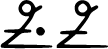
\includegraphics[scale=0.25]{././img/gaka.png}\\happiness\\contentedness} & 
					 \makecell{
\includegraphics[scale=0.25]{././img/gapoka.png}\\pleasure\\(not nec. sexual)} & 
					 \makecell{
\includegraphics[scale=0.25]{././img/gangaka.png}\\unhappiness\\discontent\\sadness, anger(strong)} & 
					 \makecell{
\includegraphics[scale=0.25]{././img/gangapoka.png}\\pain\\displeasure} \\
				 \emph{-ti} & 
					 \makecell{
\includegraphics[scale=0.25]{././img/gati.png}\\affection\\(often romantic)} & 
					 \makecell{
\includegraphics[scale=0.25]{././img/gapoti.png}\\lust\\wanting, craving} &
					 \makecell{
\includegraphics[scale=0.25]{././img/gangati.png}\\disdain\\detest(stronger)} &
					  \makecell{
\includegraphics[scale=0.25]{././img/gangapoti.png}\\repulsion\\disgust} \\
				 \emph{-\W u} & 
					 \makecell{
\includegraphics[scale=0.25]{././img/gawu.png}\\confidence} &
					 \makecell{
\includegraphics[scale=0.25]{././img/gapowu.png}\\courage} &
					 \makecell{
\includegraphics[scale=0.25]{././img/gangawu.png}\\doubt\\anxiety} &
					 \makecell{
\includegraphics[scale=0.25]{././img/gangapowu.png}\\fear} \\
				 \emph{-t\OO} &
					 \makecell{
\includegraphics[scale=0.25]{././img/gato.png}\\excitement} &
					 \makecell{
\includegraphics[scale=0.25]{././img/gapoto.png}\\arousal} &
					 \makecell{
\includegraphics[scale=0.25]{././img/gangato.png}\\dissapointment} &
					 \makecell{
\includegraphics[scale=0.25]{././img/gangapoto.png}\\helplessness}\\
				 \emph{-xa} &
					 \makecell{
\includegraphics[scale=0.25]{././img/gaxa.png}\\pride} &
					 \makecell{
\includegraphics[scale=0.25]{././img/gapoxa.png}\\acceptance\\self of belonging} &
					 \makecell{
\includegraphics[scale=0.25]{././img/gangaxa.png}\\shame} &
					 \makecell{
\includegraphics[scale=0.25]{././img/gangapoxa.png}\\reclusiveness\\lack of belonging} \\ \hline
				\end{tabular}
			\end{table}

		\subsubsection{TARG}
			The TARG suffixes indicate the target of the emotion. There are four possibilities for this morphosyntactic category:
				\begin{itemize}
					\item -\emph{xu} represents an animate target. This can be a person or an animal (anything with consciousness).
					\item -\emph{\F u} represents no target. It is also the inanimate suffix for a lot of constructions, and it can serve that purpose here too (eg: mad at your washing machine), but an inanimate pronoun usually follows to provide context in an ambiguous environment.
					\item -\emph{mu} is a reflexive target.
					\item -\emph{\R u} is a reciprocal target.
				\end{itemize}

			\begin{figure}[H] % Interlineraization examples go here.
			\label{interlin_emo_targ}

				\begin{example}
				\label{ex:interlin_emo_targ_1}
					Gakaxu si. [ga.\stress ka.xu.si]
					\gll ga -ka -xu si
					emotional -\D{emo:content} -\D{targ:anim} \cop
					\glt `I am content (with someone).'
					\glend
				\end{example}

				\begin{example}
				\label{ex:interlin_emo_targ_2}
					Gakafu si. [ga.\stress ka.\F u.si]
					\gll ga -ka -\F u si
					emotional -\D{emo:content} -\D{targ:null} \cop
					\glt `I am content.'
					\glend
				\end{example}

				\begin{example}
				\label{ex:interlin_emo_targ_3}
					Gakamu si. [ga.\stress ka.mu.si]
					\gll ga -ka -mu si
					emotional -\D{emo:content} -\D{targ:refl} \cop
					\glt `I am content (with myself).'
					\glend
				\end{example}

				\begin{example}
				\label{ex:interlin_emo_targ_4}
					Gakaru si. [ga.\stress ka.\R u.si]
					\gll ga -ka -\R u si
					emotional -\D{emo:content} -\D{targ:recip} \cop
					\glt `I am am in a state of mutual content with another person.' % Is there a better way to gloss this? lol...
					\glend
				\end{example}
			\caption{Examples of emotional constructions using different TARG suffixes}
			\end{figure}

		\subsubsection{DUR}
			DUR suffixes are often omitted in common conversation, and used primarily to parse apart the subtle differences between discrete emotions.
				\begin{itemize}
					\item The long durative -\emph{da} indicates that the emotion occurred for a long period of time, something like the distinction between an emotion and a mood.
					\item The short durative -\emph{pa}, on the other hand, marks the emotion as a fleeting state.
				\end{itemize}

			\begin{figure}[H] % Interlineraization examples go here.
			\label{interlin_emo_dur}

				\begin{example}
				\label{ex:interlin_emo_dur_1}
					Gatirupa si. [ga.\stress ti.\R u.pa.si]
					\gll ga -ti -\R u -pa si
					emotional -\D{emo:affection} -\D{targ:recip} -\D{dur:short} \cop
					\glt `I am in love.' (fleeting)
					\glend
				\end{example}

				\begin{example}
				\label{ex:interlin_emo_dur_2}
					Gatiruda si. [ga.\stress ti.\R u.da.si]
					\gll ga -ti -\R u -da si
					emotional -\D{emo:affection} -\D{targ:recip} -\D{dur:long} \cop
					\glt `I am in love.' (longstanding)
					\glend
				\end{example}

			\caption{Examples of emotional constructions using different DUR suffixes}
			\end{figure}

	\subsection{Reduplication}
		Like other morphological categories in {\kurango}, EMO, DUR, TARG, PRIM, NEUT, and NEG can be reduplicated in order to modify intensity. It is interesting to note that reduplicating the PRIM suffix creates the lexicalized expression akin to the word ``fuck'' in English in terms of distribution and meaning. Etymologically, this comes from expressions like (\ref{ex:interlin_emo_prim_2}), which is the most common usage of \emph{po}.



	\section{Numeracy}

	\subsection{The cardinal root \emph{\R\OO}}
		Cardinal numbers in {\kurango} are marked with the cardinal root \emph{\R\OO}. The vowel can be lengthened to form \emph{\R\OO\OO}, ``number'' as an abstract concept. However, it more commonly appears with the numeracy suffixes, discussed below.
	\subsection{Numeracy suffixes}
		\kurango 's capacity to encode any number comes from the combination of ten morphemes that represent the numbers 0-9. These morphemes have underlying forms that obey syllable structure rules for \kurango, but they are commonly discussed as though they only have consonants in their stems. This is because of an overarching vowel harmony rule based on whether or not the initial numeral suffix is odd or even (see below). 
		% couldn't get autoref to properly work here
			\begin{table}[H]
			\centering
			\caption{{\kurango} numeracy suffixes}
			\label{numeracy_table}
				\begin{tabular}{c|ccc}
					Numeral & Suffix & -a glyph & -u glyph \\ \hline\hline
					1 & -xa\R a & 
						
\includegraphics[scale=0.25]{././img/1A.png} &
						
\includegraphics[scale=0.25]{././img/1U.png} \\
					2 & -duzu &
						
\includegraphics[scale=0.25]{././img/2A.png} &
						
\includegraphics[scale=0.25]{././img/2U.png} \\
					3 & -ta\R a &
						
\includegraphics[scale=0.25]{././img/3A.png} &
						
\includegraphics[scale=0.25]{././img/3U.png} \\
					4 & -kutu &
						
\includegraphics[scale=0.25]{././img/4A.png} &
						
\includegraphics[scale=0.25]{././img/4U.png} \\ 
					5 & -sa\N a &
						
\includegraphics[scale=0.25]{././img/5A.png} &
						
\includegraphics[scale=0.25]{././img/5U.png} \\
					6 & -zusu &
						
\includegraphics[scale=0.25]{././img/6A.png} &
						
\includegraphics[scale=0.25]{././img/6U.png} \\
					7 & -sata &
						
\includegraphics[scale=0.25]{././img/7A.png} &
						
\includegraphics[scale=0.25]{././img/7U.png} \\
					8 & -\glot u\glot u &
						
\includegraphics[scale=0.25]{././img/8A.png} &
						
\includegraphics[scale=0.25]{././img/8U.png} \\
					9 & -na\B a &
						
\includegraphics[scale=0.25]{././img/9A.png} &
						
\includegraphics[scale=0.25]{././img/9U.png} \\
					0 & -zu\R u &
						
\includegraphics[scale=0.25]{././img/0A.png} &
						
\includegraphics[scale=0.25]{././img/0U.png} \\ \hline
				\end{tabular}
			\end{table}

		So, \emph{roxara} would gloss to ``one,'' but these suffixes can also attach to nouns. An example would be \emph{o'atikutu}, or "four dogs."

		\subsubsection{Larger numbers and vowel harmony}
		\label{number_harmony}
			A language should, naturally, have a way to discuss really large numbers. In \kurango, this is as simple as attaching multiple suffixes to \emph{\R\OO}. However, there is a catch:

				\begin{figure}[H]
				\label{interlin_num_harm}
					\begin{example}
					\label{num_a_harm}	
						roxarazarasata [\R\OO.\stress xa.\R a.za.\R a.sa.ta]
						\gll {\R\OO} -xa\R a -zu\R u -sata
						\D{num} -one -zero -seven
						\glt `one hundred seven'
						\glend
					\end{example}

					\begin{example}
					\label{num_u_harm}
						*roxarazurusata [\R\OO.\stress xa.\R a.zu.\R u.sa.ta]
						\gll {\R\OO} -xa\R a -zu\R u -sata
						\D{num} -one -zero -seven
						\glt `(Intended) one hundred seven'
						\glend
					\end{example}
				\end{figure}

			As stated earlier, there is an overarching vowel harmony rule based on whether or not the initial numeral suffix is odd or even. Looking at the numeracy suffixes above, a noticeable pattern emerges, where odd numeral suffixes have /a/ as their vowels and even numeral suffixes (and zero) have /u/ as their vowels. The suffix that attaches closest to the root \emph{\R\OO} determines the vowel harmony for the rest of the numeral construction.

	\subsection{Ordinality}
		Ordinality in {\kurango} is a lot more simple than English ordinality. There are no semantic classes of objects that take different ordinal morphology (take ``tertiary'' versus ``third'')---all take the same derivational suffix \emph{-ta}. For example, \emph{o'atitakutu} would translate to ``the fourth dog'' (compare with \emph{o'atikutu} ``four dogs'' above).

		\subsubsection{Ordinality and calendar terms}
			The ordinal suffix is used on the roots ``year,'' ``day,'' ``week,'' and ``month'' to express calendar terms.

			\begin{itemize}
			\item \emph{di} is the root for ``day.'' \emph{ditaxa\R ana\B a} would translate to ``the nineteenth day,'' and \emph{dixa\R ana\B a} to ``nineteen days.''

			\item \emph{\glot u} is the root for ``week.'' \emph{\glot uta\glot u\glot uzu\R u} would translate to ``the eightieth week,'' and \emph{\glot u\glot u\glot uzu\R u} to ``eighty weeks.''

			\item \emph{m\OO} is the root for ``month.'' \emph{m\OO tata\R a} would translate to ``March (lit: the third month),'' and \emph{m\OO ta\R a} to ``three months.''

			\item \M i is the root for ``year.'' \emph{\M itaduzuzu\R uxu\R usu\N u} would translate to ``2015 (lit: the 2015th year),'' and \emph{\M iduzuzu\R uxu\R usu\N u} to ``2015 years.''
			\end{itemize}

	\subsection{Multiplicative adverbs}
		Cardinal number constructions can be derived into multiplicative adverbs ``double, triple, quadruple'' as they can in English, using an additional root that is mutually exclusive with the noun slot. This root is \emph{d\OO\R\OO}. An example would be \emph{d\OO\R\OO sata}, which translates to ``septuple.''

	\subsection{Morphosyntax}
		\begin{table}[H]
		\centering
		\label{num_morphosyntax}
			\begin{tabular}{cccc}
			Root & Slot 1 & Slot 2 & Slot 3-$\infty$ \\ \hline\hline
			\makecell{\R\OO\\d\OO\R\OO\\any noun} & \makecell{-ti\\
			%-d\OO THIS WAS IN THIS SLOT ALSO, WHAT DOES IT MEAN
			} & \makecell{Numeracy suffix\\(that determines vowel harmony)} & \makecell{Numeracy suffix\\(that undergoes vowel harmony)} \\ \hline
			\end{tabular}
			\caption{Morphosyntax of numeracy constructions}
		\end{table}

	\subsection{Other useful numeracy constructions}
		There are several other common constructions where numeracy suffixes come in handy.

		\begin{itemize}
			\item Last names: \emph{\glot a\N ataduzu} ``last name (lit: second name)''
			\item Secondary emotions: \emph{gatitixu si ga\N a\W u\F upataduzu si} ``I love someone, but I am also scared (lit: I love someone; my second emotion is fear)'' % May not be grammatically correct. Possibly missing something like ``but''
		\end{itemize}

% Dont forget: lengthening of last vowel for turning a morpheme into a noun.

% Talk about unlimited (virtually?) zero derivation

 % morphology
	\documentclass[12pt]{article}
	%FORMATTING
		\usepackage{graphicx} %op shit
		\usepackage[margin=1in]{geometry} %Set margins
		\usepackage{fixltx2e} %subscript
	%LINGUISTICS-RELATED PACKAGES
		\usepackage{qtree} %syntax trees
		\usepackage{covington} %interlinearizations
		\usepackage{amsmath,amsthm,amssymb} %empty set and some other shit
		\usepackage{tipa} %ipa

	\let\oldemptyset\emptyset %Redefines the shitty empty set symbol to the old one.
	\let\emptyset\varnothing

	%stuff for handling how awful it is to use default tipa syntax
		\newcommand{\R}{\textipa{R}} %alv tap
		\newcommand{\N}{\textipa{N}} %eng
		\newcommand{\OO}{\textipa{O}} %open o, DONT FORGET THE SECOND O!!!
		\newcommand{\B}{\textipa{B}} %bilab fric voi
		\newcommand{\G}{\textipa{G}} %velar fric voi
		\newcommand{\W}{\textturnmrleg} %velar approximant
		%\textipa{:}

		\newcommand{\0}{$\emptyset$} %Null
		\newcommand{\D}{\scshape} %smallcaps

		\newcommand{\kurango}{K\textipa{uRaNO}}
		\newcommand{\nom}{\D{nom}}
		\newcommand{\erg}{\D{erg}}
		\newcommand{\abs}{\D{abs}}
		\newcommand{\gen}{\D{gen}}
		\newcommand{\poss}{\D{poss}}
		\newcommand{\emo}{\D{emo}}
		\newcommand{\cop}{\D{cop}}
		\newcommand{\caus}{\D{caus}}
		\newcommand{\pst}{\D{pst}}
		\newcommand{\fut}{\D{fut}}

%--------------------------------------------------------------%
%  EXAMPLE INTERLINEAR GLOSS, ADAPTED FROM LEV'S DISSERTATION  
%															   
%	\begin{example}											   
%	\label{ex:nasalpoa}										   
%		Ontagake. \textipa{[ontagakse]}						   
%		\gll o= n- tag -ak -e 								   
%		3nmS= irreal burn -perf -irreal.i 					   
%		\glt `It will burn.' 								   
%		\glend 												   
%	\end{example} 											   
%  															   
%	%Reference examples like this: (\ref{ex:nasalpoa})         
%--------------------------------------------------------------%

%This is a test\footnote{This is not a test; it's an example of a footnote.}

\begin{document}
\title{Example Ku\textipa{RaNO} sentences interlinearized}
\maketitle

	\section{Valence-increasing morphology}
		\subsection{Applicatives}
			Applicatives in {\kurango} are marked using a suffix on the introduced argument, -\textipa{P}uti.
			\begin{example}
			\label{ex:nonapplicative}
				Nimotivagaana. \textipa{[nimOtiBaga:na]}
				\gll ni- {\0-} m\OO ti -\B a -ga\textipa{:} -na -\0
				2- {\erg-} die -{\D{caus}} -{\D{fut}} -1 -\abs
				\glt `You are going to kill me.'
				\glend
			\end{example}

			\begin{example}
			\label{ex:applicative}
				Nimotivagaana soodongu'uti. \textipa{[nigu naku mOtiBaga: sO:dONuPuti]}
				\gll ni- {\0-} m\OO ti -\B a -ga\textipa{:} -na -\0 {s\OO\textipa{:}d\OO} -\N u -\textipa{P}uti
				1- {\erg}- kill -{\caus} -{\fut} -1 -{\abs} sword {-\gen} -{\D{appl}}
				\glt `You are going to kill me with a sword.' (lit: `You made me die with a sword.')
				\glend
			\end{example}

		\subsection{Causatives}
			Causatives in {\kurango} are marked using the verbal suffix -\B a.

			\begin{example}
			\label{ex:noncausative}
				Nakumotigaa. \textipa{[nakumOtiga:]}
				\gll na- ku- m\OO ti -ga\textipa{:}
				{\D{1}}- {\D{nom}}- die -{\D{fut}}
				\glt `I am going to die.'
				\glend
			\end{example}

			\begin{example}
			\label{ex:causative}
				Namotivagaana. \textipa{[namOtiBaga:na]}
				\gll na- {\0-} m\OO ti -\B a -ga\textipa{:} -na -\0
				{\D{1}} {\D{erg}}- die -{\D{caus}} -{\D{fut}} -1 -\abs
				\glt `I am going to kill myself.' (lit: `I am going to make myself die.')
				\glend
			\end{example}

		If an agentive argument is not introduced with the causative suffix -\B a, the utterance is still grammatical, but it has a passivized 
		%what should i call this??
		 connotation to it.

		 	\begin{example}
		 	\label{ex:noncausative}
		 		Nakumotivagaa. \textipa{[nakumOtiBaga:]}
		 		\gll na- ku- m\OO ti -\B a -ga\textipa{:}
		 		1- {\nom-} die {-\caus} {-\fut}
		 		\glt `I am going to be killed' (lit: I am going to be made dead) %Is this future perfect or just future? wtf
		 		\glend
		 	\end{example}



	\section{Valence-decreasing morphology}

	\section{Directionals}

	\section{Case assignment}
		Ku\R a\N\OO 's case system can be described as ``fluid-S,'' in that arguments of intransitive verbs (S) pattern either with subjects of transitive verbs (S\textsubscript{A}) or objects of transitive verbs (S\textsubscript{O}). Determining the way in which S patterns has to do with the semantics of the utterance: S\textsubscript{A} (marked with {\D{nom}} on the Agent) has no entailment about the volition of the Agent in the action being performed, while S\textsubscript{O} (marked with {\D{erg}} on the Agent) entails that the agent was volitional in the action being performed.

		\begin{example}
		\label{ex:case_erg}
			Nakari. [naka\R i]
			\gll na- \0- ka\R i
			{\D{1}}- {\D{erg}}- sleep
			\glt `I sleep.' (by my own volition.)
			\glend
		\end{example}

		\begin{example}
		\label{ex:case_abs}
			Nakukari. [nakuka\R i]
			\gll na- ku- ka\R i
			{\D{1}}- {\D{nom}}- sleep
			\glt `I sleep.' (no entailment about my volition.)
			\glend
		\end{example}

		\subsection{Case assignment in transitive sentences}
			Case assignment of (lexically) transitive verbs is similar to that of English. Agents take {\D{nom}} case, and Themes(Objects) take {\D{acc}} case. In ditransitives, {\D{gen}} case is also used on the second Object(Instrument/Beneficiary/Recipient/etc), as in (\ref{ex:case_ditrans}).

			\begin{example}
			\label{ex:case_ditrans}
				Nawivinu namiromiku nungu. \textipa{[na\W i\B inu nami\R\OO miku nu\N u]}
				\gll na- \0- \W i\B i -nu {-\0} na- {mi\R\OO} -mi -ku nu -\N u
				1- \erg- give -3 {-\abs} 1- cat {-\poss} {-\abs} 3 -\gen
				%is case assignment in this sentence OK?
				\glt `I give him/her my cat.'
				\glend
			\end{example}
				%\begin{example}
				%\label{ex:case_ditransitive}
				%	Naku namiromirhu wivi nungu. \textipa{[naku nami\R\OO mi\G u \W i\B i nu\N u]}
				%	\gll na -ku na- {mi\R\OO} -mi -\G u \W i\B i nu -\N u
				%	1 -{\D{nom}} 1- cat -{\D{poss}} -{\D{acc}} give {\D{3}} -{\D{gen}}
				%	\glt `I gave him/her my cat.'
				%	\glend
				%\end{example}

			\subsubsection{Case assignment in causatives}
				In a causative sentence, fluidity of S is preserved (as the verb is underlyingly intransitive), which once again has entailment for the Agent's volition in the action being performed. {\D{erg}} case-marking on the Agent entails that the agent is volitional in the action being performed (as in (\ref{ex:fluids_erg})). {\D{nom}} case-marking has no implication about the agent's volition in the action being performed (as in (\ref{ex:fluids_abs})). 
				%Case-marking on the Theme and Instrument also vary based on how the Agent's case is marked.
					%OR
				%Themes always take \D{acc} case-marking and Instruments always take \D{gen} case-marking, regardless of how case is marked on the Agent.
					%WHICH OF THESE IS TRUE LOL

				\begin{example}											   
				\label{ex:fluids_erg}										   
						Gangaka nasivamonu. \textipa{[gaNaka nasiBamOnu]}
						\gll ga -\N a -ka na- \0- si -\B a {-m\OO} -nu -\0						   
			   			{\emo} -{\D{neg}} -{\D{emo:happy}} 1- {\erg-} {\cop} {-\caus} {-\pst} 3 -\abs
						\glt `I made him/her unhappy.' (It is my fault that he/she was unhappy.) 								   
						\glend 												   
				\end{example}

				\begin{example}
				\label{ex:fluids_abs}
						Gangaka nakusivamonu. \textipa{[gaNaka nakusiBamOnu]}
						\gll ga -\N a -ka na- ku- si -\B a {-m\OO} -nu -\0				   
			   			{\emo} -{\D{neg}} -{\D{emo:happy}} 1- {\nom}- {\cop} {-\caus} {-\pst} 3 -\abs
						\glt `I made him/her unhappy.' (No implication that it was my fault.)
						\glend
				\end{example}

			\subsubsection{Negation and case assignment in causative verbs: semantic implications}
				%What is actually being negated??? help

\end{document}

 % interlinearizations chapter
	\chapter{Orthography}
\label{chap:ortho}

HOW DO I TYPESET THIS????

\section{Handwritten \emph{kuraito}}

\section{Romanization of \kurango}
	Since the formal \emph{kuraito} script can be inconvenient at times to write (as can IPA), {\kurango} is often written using the Roman alphabet, accomplishable on any standard English keyboard. This romanization standard is used in the dictionary (\autoref{chap:dict}).

	\begin{table}[H]
	\centering
	\label{roman}
		\begin{tabular}{cc}
		Original IPA & Romanized equivalent \\ \hline\hline
		\F & f \\
		\B & v \\
		\W & w \\
		\R, \textipa{\*r} & r \\
		\N & ng \\
		\G & rh \\
		\M & j \\ 
		\OO & o \\ \hline
		\end{tabular}
	\caption{Romanization standards for \kurango}
	\end{table}


	\begin{appendices}
		%\entry{Ortho}{IPA}{Partofspeech}{Definition}

%Weird glitches involving columns. look into the package and if that wont do it then do some janky shit to it.

\chapter{Dictionary}
\label{chap:dict}

\section*{A}
\begin{multicols}{2}
	\entry{adara}{\glot a.\stress da.\R a}{verb}{to order. Borrowed from English name ``Adele.''}

	\entry{afa}{\stress\glot a.\F a}{interjection}{yes. Designed to be maximally phonetically distinct from \emph{i'i}, ``no.''}

	\entry{a'i}{\stress\glot a.ji}{noun, determiner}{space, location. As a determiner functions similarly to English ``where.''}

	\entry{a'iramoo}{a.\stress ji.\R a.m\OO\len}{noun}{outsider, alien, outgroup member (pejorative)}

	\entry{anga}{\stress\glot a.\N a}{noun}{name}

	\entry{ari}{\stress\glot a.\R i}{verb}{to go}
\end{multicols}

\section*{B}
\begin{multicols}{2}
	%\entry{Ortho}{IPA}{Partofspeech}{Definition}
	\entry{bako}{\stress ba.k\OO}{noun}{body. Often compounds to form different parts of the body, e.g. \emph{vafawaabako} ``mouth.''}

	\entry{bo'i}{bji}{determiner}{how, by}

	\entry{boraa}{b\OO.\stress\R a\len}{inf. morpheme}{progressive aspect marker. Historically served as a present tense marker but that is now null.}
\end{multicols}

\section*{D}
\begin{multicols}{2}
	\entry{-da}{da}{infl. morpheme}{emotion marker for long duration}

	\entry{di}{di}{noun}{day. Borrowed from English ``day.''}

	\entry{doro}{\stress d\OO.\R\OO}{adverb}{multiplicative adverb. Compare to English ``-tuple'' morph.}

	\entry{duru}{\stress du.\R u}{verb}{to follow. Borrowed from English name ``Dora.''}

	\entry{duzu}{\stress du.zu}{quantifier}{two. Borrowed loosely from French \emph{deux}, ``two.''}

\end{multicols}

\section*{F}
\begin{multicols}{2}
	\entry{-fa}{fa}{infl.morpheme}{marks a target as proximal} % IS THIS A PREPOSITION?

	\entry{faavu}{\stress\F a\len.\B u}{noun}{home}

	\entry{fivu}{\stress\F i.\B u}{noun}{house}

	\entry{-fu}{\F u}{infl. morpheme, pronoun}{marks an inanimate target.  Also serves as the emotion marker for an inanimate target.}
\end{multicols}

\section*{G}
\begin{multicols}{2}
	\entry{ga}{ga}{adjective}{emotional}

	\entry{-gaa}{ga\len}{infl. morpheme}{future tense marker}

	\entry{gaaro}{\stress ga\len.\R\OO}{verb}{select}

	\entry{gakagangasiri}{\stress ga.ka.\stress ga.\N a.\stress si.\R i}{interjection}{lexicalized expression means ``How are you?'' Literally translates to ``*Good emotion, bad emotion, is it?''}

	\entry{gaka}{\stress ga.ka}{adjective}{lexicalized expression that means ``good.'' Literally means ``good emotion.''}

	\entry{gakasi}{ga.\stress ka.si}{interjection}{lexicalized expression that means ``Hello.'' Literally translates to ``*Emotion is good.''}

	\entry{ganga}{\stress ga.\N a}{adjective}{lexicalized expression that means ``bad.'' Literally translates to ``*negated emotion.''}

	\entry{gangasi}{ga.\stress\N a.si}{interjection}{lexicalized expression that means ``Hello.'' Literally translates to ``*Emotion is negated.''}

	\entry{go'i}{\stress g\OO .\glot i}{verb}{to desire, want}

	\entry{goo}{g\OO\len}{preposition}{ablative preposition; ``from''}

	\entry{gokoo}{\stress g\OO.k\OO\len}{preposition}{illative preposition; ``into, back from''}

	\entry{gooko}{\stress g\OO\len.k\OO}{preposition}{departative preposition; ``leave (with intention of returning).''}

\end{multicols}

\section*{I}
\begin{multicols}{2}
	\entry{i'a}{\stress i.ja}{preposition}{oblique preposition; ``east of''}

	\entry{i'i}{\stress\glot i.ji}{interjection}{no. Designed to be maximally phonetically distinct from \emph{afa}, ``yes.''}

	\entry{inakara}{\glot i.\stress\N a.ka.\R a}{verb}{to bore. Borrowed from English surname ``Inkelas.''}
\end{multicols}

\section*{J}
\begin{multicols}{2}
	\entry{-ja}{\M a}{deriv. morpheme}{serves as a person marker (example: ``learn'' to ``learner''). Changes word class from verb to noun.}

	\entry{ji}{\M i}{noun}{year. Borrowed loosely from English ``year.''}

	\entry{jivi}{\stress\M i.\B i}{verb}{give. Borrowed loosely from English ``give.''}

\end{multicols}

\section*{K}
\begin{multicols}{2}
	\entry{-ka}{ka}{deriv. morpheme}{emotion marker for ``happiness.'' Changes word class from noun to adjective.}

	\entry{kanga}{\stress ka.\N a}{infl. morpheme}{perfective marker. Combines with future and past tense markers to form past perfect and future perfect.}

	\entry{kari}{\stress ka.\R i}{verb}{to sleep. Truncated form of Japanese name \emph{\begin{CJK}{UTF8}{min}紫\end{CJK}} ``Yukari.''}

	\entry{karipa}{ka.\stress\R i.pa}{verb, noun}{to nap, a nap. Exocentric compound of \emph{kari} ``to sleep'' and \emph{pa}, the short emotion durative.}

	\entry{kii}{ki\len}{noun, determiner}{time. As a determiner, functions similarly to English ``when.''}

	\entry{kogoo}{\stress k\OO.g\OO\len}{preposition}{elative preposition; ``from, out of''}

	\entry{koo}{k\OO\len}{preposition}{allative preposition; ``to''}

	\entry{koogo}{\stress k\OO\len.g\OO}{preposition}{redepartitive preposition, ``come with intention of leaving''}

	\entry{koogoo}{\stress k\OO\len .g\OO\len}{preposition}{preposition that means ``to and from.'' An echo construction based on prepositions \emph{koo} ``to'' and \emph{goo} ``from.''} % get a better gloss for this...

	\entry{kopanga}{k\OO.\stress pa.\N a}{noun}{friend, borrowed from French \emph{copain}}

	\entry{ku'a}{kwa}{noun}{time}

	\entry{kura}{\stress ku.\R a}{noun}{brain}

	\entry{kura}{\stress ku.\R a}{verb}{to think}

	\entry{kura'ito}{ku.\stress\R a.ji.t\OO}{noun}{writing} % make sure u add more info on the etymology of this later as it IS a compound word.

	\entry{kuraja}{ku.\stress\R a.\W a}{noun}{person. Excocentric compound of ``think'' and person marker---literally ``thinker.''}

	\entry{kurango}{ku.\stress\R a.\N\OO}{noun}{language} % make sure u add more info on the etymology of this later as it IS a compound word.

	\entry{kutu}{\stress ku.tu}{quantifier}{four. Borrowed loosely from French \emph{quatre}, ``four.''}
\end{multicols}

\section*{M}
\begin{multicols}{2}
	\entry{-mi}{mi}{determiner}{posessive pronoun marker. Borrowed from English ``my.'' Assigns genitive case.}

	\entry{miro}{\stress mi.\R\OO}{noun}{cat. Borrowed from English name ``Milo.''}

	\entry{-miiti'a}{\stress mi\len.tja}{deriv. morpheme}{sensation suffix for sense (as in, a sixth, holistic sense). Last vowel can be lengthened to mean ``sensation.'' Commonly affixed to the evidential clitic \emph{kixada}.}
	
	\entry{mo}{m\OO}{noun}{month. Borrowed loosely from English ``month.''}

	\entry{-mo}{m\OO}{infl. morpheme}{past tense marker}

	\entry{moti}{\stress m\OO .ti}{verb}{to die. Borrowed loosely from French \emph{mourir} ``die.''}

	\entry{-mu}{mu}{infl. morpheme}{emotion marker for a reflexive target}

	\entry{-muzu}{\stress mu.zu}{deriv. morpheme, pronoun}{reflexive pronoun. Lowers valency of verb.}
\end{multicols}

\section*{N}
\begin{multicols}{2}
	\entry{na}{na}{determiner}{first person marker}

	\entry{na'isaguu}{noun}{na.\stress ji.sa.gu\len}{dog food (ketchup)}

	\entry{nana}{\stress na.na}{determiner}{first person pronoun. Reduplcation of \emph{na}, the first person marker.}

	\entry{nava}{\stress na.\B a}{quantifier}{nine. Borrowed loosely from French \emph{neuf}, ``nine.''}

	\entry{ni}{ni}{determiner}{second person marker}

	\entry{nini}{\stress ni.ni}{determiner}{second person pronoun. Reduplication of \emph{ni}, the second person marker.}

	\entry{no'a}{\stress n\OO.ja}{preposition}{oblique preposition; ``north of''}

	\entry{-no'i}{\stress n\OO.ji}{deriv. morpheme}{emotion marker for a neutered emotion}

	\entry{noriga}{n\O.\stress\R i.ga}{noun}{Norway. Borrowing of Norwegian \emph{Norge}.}

	\entry{nu}{nu}{determiner}{third person marker}

	\entry{-numungu}{nu.\stress mu.\N u}{deriv. morpheme}{sensation suffix for smell. Last vowel can be lengthened to mean ``smell.'' Commonly affixed to the evidential clitic \emph{kixada}. Etymologically derived from association of nasal consonants and smell.}

	\entry{nunu}{\stress nu.nu}{determiner}{third person pronoun. Reduplication of \emph{nu}, the third person marker.}
\end{multicols}

\section*{NG}
\begin{multicols}{2}
	\entry{nga}{\N a}{deriv. morpheme}{negation morpheme}

	%\entry{ngu}{\N u}{infl. morpheme, pronoun}{genitive marker} %DO i even still use this???

	\entry{-nga'uva}{\N a.\stress ju.\B a}{deriv. morpheme}{changes word class from verb to noun} % Is this even ``legal?'' What else should this do? Semantically related to -nga and -va

	\entry{-ngo}{\N\OO}{deriv. morpheme}{sensation suffix for sound, language. Last vowel can be lengthened to mean ``sound.'' Commonly affixed to the evidential clitic \emph{kixada}.}

\end{multicols}

\section*{O}
\begin{multicols}{2}
	\entry{o'ati}{\textipa{PO.\stress wa.ti}}{noun}{dog. Borrowed loosely from English name ``Archie.''}

	\entry{ora}{\stress\glot\OO.\R a}{verb}{to punch. Borrowing of Japanese onomatopoeia \emph{\begin{CJK}{UTF8}{min}オラ\end{CJK}}.}
\end{multicols}

\section*{P}
\begin{multicols}{2}
	\entry{-pa}{pa}{infl. morpheme}{emotion marker for short duration}

	\entry{pada}{\stress pa.da}{noun}{length. Exocentric compound of \emph{pa} and \emph{da}, the emotion duratives.}

	\entry{papi'a}{pa.\stress pja}{noun}{paper. Borrowing of English ``paper.''}

	\entry{-po}{p\OO}{deriv. morpheme}{emotion marker for a ``primal'' emotion} % Explain the semantics? Reference the emotion section?
\end{multicols}

\section*{R}
\begin{multicols}{2}
	\entry{ra'isaa}{\R a.\stress ji.sa\len}{adjective}{superfluous} % What is the etymology of this?

	\entry{ri}{\R i}{particle}{interrogative statement marker}

	\entry{-riiti}{\stress\R i\len.ti}{deriv. morpheme}{sensation suffix for sight. Last vowel can be lengthened to mean ``sight.'' Commonly affixed to the evidential clitic \emph{kixada}. Borrowed from English ``light.''}

	\entry{ro}{\R\OO}{particle}{imperative statement marker}

	\entry{ro-}{\R\OO}{quantifier}{numeracy marker. Serves as the beginnign morpheme for a cardinal number.}

	\entry{roodo}{\stress\R\OO\len.d\OO}{noun}{road. Borrowed from English ``road.''}

	\entry{-ru}{\R u}{infl. morpheme}{emotion marker for a reciprocal target}

	\entry{-ruzu}{\stress\R u.zu}{deriv. morpheme}{reciprocal morpheme. Lowers verb valency.}
\end{multicols}

\section*{RH}
\begin{multicols}{2}
	\entry{rhamuzu}{\G a.\stress mu.zu}{noun}{introspective knowledge. Lexicalization of \emph{\G a} morpheme and the reflexive \emph{-muzu}.}

	\entry{rhana}{\stress\G a.na}{verb}{to know. Used as a general expression.}

	\entry{rhangakaja}{\G a.\stress\N a.ka.\M a}{noun}{a type of knowledge used specifically in instances where the knowledge is irrelevant to the discourse. Loose borrowing of Japanese name \emph{\begin{CJK}{UTF8}{min}羽川\end{CJK}}``Hanekawa''.}

	\entry{rhanarhaa}{\G a.\stress na.\G a\len}{noun}{a type of worldly, difficult-to-obtain knowledge; a high compliment. Etymologically derived from reanalyzed reduplication of the \emph{\G a} cran-morph.}

	\entry{rhapapi'a}{\G a.\stress pa.pja}{noun}{fact-based knowledge. Lexicalization of \emph{\G a} morpheme and \emph{papi'a} ``paper.''}

	\entry{rhasotorii}{\G a.\stress s\OO.t\OO.\R i\len}{noun}{social knowledge. Inspired by English ``street smarts.''}

	\entry{-rhu}{-\G u}{determiner}{dative case marker. Used on indirect objects in ditransitive sentences.}

\end{multicols}

\section*{S}
\begin{multicols}{2}
	\entry{sa'a}{\stress sa.ja}{preposition}{oblique preposition; ``south of''}

	\entry{sanga}{\stress sa.\N a}{quantifier}{five. Loosely borrowed from French \emph{cinq}, ``five.''}

	\entry{saru}{\stress sa.\R u}{verb}{to be able to do something. A modal similar to English ``can.''}

	\entry{sata}{\stress sa.ta}{quantifier}{seven. Loosely borrowed from French \emph{sept}, ``seven.''}

	\entry{si}{si}{verb}{copula. Similar in meaning to English ``to be.''}

	\entry{soodo}{\stress s\OO\OO .d\OO}{noun}{sword. Borrowed from English ``sword.''}

	\entry{-so}{s\OO}{deriv. morpheme}{changes word class from noun to adjective}

	\entry{sotorii}{s\OO.\stress t\OO.\R i\len}{noun}{street. Borrowing of English ``street.''}

	\entry{-su}{su}{deriv. morpheme}{changes word class from verb to adjective}

	\entry{susu}{\stress su.su}{quantifier}{six. Loosely borrowed from French \emph{six}, ``six.''}

	\entry{sutaku}{su.\stress ta.ku}{verb}{to posess multiple earlobes. Loosely borrowed from English surname ``Stockdale.''}

\end{multicols}

\section*{T}
\begin{multicols}{2}
	\entry{-ta}{ta}{deriv. morpheme}{ordinality marker}

	\entry{tara}{\stress ta.\R a}{quantifier}{three. Loosely borrowed from French \emph{trois}, ``three.''}

	\entry{-ti}{ti}{deriv. morpheme}{emotion marker for ``affection.'' Changes word class from noun to adjective.}

	% Theres also a -ti plural morph, but may be obsoleted by opposite edge reduplication process. Maybe only for monosyllabic roots?

	\entry{-to}{t\OO}{deriv. morpheme}{emotion marker for ``excitement.'' Changes word class from noun to adjective.}

	\entry{-tuusi}{\stress tu\len.si}{deriv. morpheme}{sensation suffix for touch. Last vowel can be lengthened to mean ``touch.'' Commonly affixed to the evidential clitic \emph{kixada}. Loosely borrowed from English ``touch.'' Can be negated to mean ``pain'' (\emph{ngatuusii}).}
\end{multicols}

\section*{U}
\begin{multicols}{2}
	\entry{u}{\glot u}{noun}{week. Borrowed loosely from English ``week.''}

	\entry{uba'a}{\glot u.\stress bja}{preposotion}{oblique preposition; ``over, above''}

	\entry{uda'a}{\glot u.\stress dja}{preposition}{oblique preposition; ``under, below''}

	\entry{usu}{\stress\glot u.su}{adverb}{also}

	\entry{uti}{\stress\glot u.ti}{deriv. morpheme}{applicative morpheme. Increases verb valency. If attached to a noun, changes class to a verb.}

	\entry{u'u}{\stress\glot u.wu}{quantifier}{eight. Borrowed loosely from French \emph{huit}, ``eight.''}
\end{multicols}

\section*{V}
\begin{multicols}{2}
	\entry{-va}{\B a}{deriv. morpheme}{causative morpheme. Increases verb valency.}

	\entry{-vafawa}{\B a.\stress\F a.\W a}{deriv. morpheme}{sensation suffix for taste. Last vowel can be lengthened to mean ``taste.'' Commonly affixed to the evidential clitic \emph{kixada}. Etymotically derived from the associaton of labial consonants and taste.}

	\entry{voru}{\stress\B\OO.\R u}{verb}{please (as in ``to please someone.'' Borrowed from the English name ``Vore.'')}
\end{multicols}

\section*{W}
\begin{multicols}{2}
	\entry{wa}{\W a}{determiner}{that, this (depending on attached morphology)}

	\entry{wa'a}{\stress\W a.ja}{preposition}{oblique preposition; ``west of''}

	\entry{wooka}{\stress\W\OO\len .ka}{deriv. morpheme, determiner}{reason clitic. Marks a subordinate clause that gives a reason for another clause. As a determiner, functions similarly to English ``why.''}

	\entry{-wu}{\W u}{deriv. morpheme}{emotion marker for ``confidence.'' Changes word class from noun to adjective.}
\end{multicols}

\section*{X}
\begin{multicols}{2}
	\entry{-xa}{xa}{deriv. morpheme}{emotion marker for ``pride.'' Changes word class from noun to adjective.}

	\entry{xara}{\stress xa.\R a}{quantifier}{one}

	\entry{xoranu}{x\OO.\stress\R a.nu}{verb}{to sweat. Borrowed loosely from English surname ``Holland.''}

	\entry{-xu}{xu}{infl. morpheme}{marker for an animate target. Also serves as the emotion marker for an animate target.}
\end{multicols}

\section*{Z}
\begin{multicols}{2}
	\entry{-za}{za}{infl. morpheme}{marks a target as distal}

	\entry{-zo}{z\OO}{deriv. morpheme}{changes word class from noun to adverb}

	\entry{-zu}{zu}{deriv. morpheme}{changes word class from verb to adverb}

	\entry{zuru}{\stress zu.\R u}{quantifier}{zero. Borrowed loosely from French \emph{zero}, ``zero.''}

\end{multicols}


  % dict chapter
		\chapter{{\kurango} Phrasebook} % kng phrasebook
		\chapter{Typesetting \kurango}
\label{chap:typeset}

{\kurango} is available for use as a set of .ttf fonts, compatable with most word processors. Because {\kurango}'s orthography is a syllabary (see \autoref{chap:ortho}), the current way it is typed is using a set of Japanese fonts (not simply one, as {\kurango} has more glyphs than standard Japanese.)

The fonts were created using \url{http://www.paintfont.com/} and Adobe Photoshop CS6. I plan to create a more better-designed font using a vector program like Adobe Illustrator in the future if I have more time/skill.

\section{Mapping onto Japanese font}
	Because {\kurango} and Japanese are very different languages, the mapping of {\kurango} onto a Japanese font is not 1:1. For example, all Japanese glyphs with a nucleus of /e/ are ignored, as {\kurango} has no /e/ phoneme. However, additional phonemes like /\N, \G, \B/, etc, needed to be added into a Japanese font which does not natively include them. 

	The way this was handled was through the use of two font types: ``Normal'' and ``Irregular.'' 

	The ``Normal'' font includes any onset that is natively found in Japanese, with the exception of /\F/, which was substituted for Japanese /h/\footnote{An allophone of Japanese /h/ is /\F/.} (but still typed using <h>). The normal font includes the onsets /\glot, k, g, s, z, t, d, n, \F, p, b, m, \R/ and the nuclei /a, i, u, \OO/ (/\OO/ is typed using <o>).

	The ``Irregular'' font includes any onset \emph{not} natively found in Japanese. This includes the onsets /x, \G, \N, \W, \B, \M/. Below is a table of how these fonts were mapped onto Japanese:
		\begin{CJK}{UTF8}{min}
		\begin{table}[H]
		\centering
		\caption{Onset mapping from Japanese to \kurango. Any form not included in the table is not included in the fonts.}
		\label{irregular_font}
			\begin{tabular}{c|cccccccc}\hline\hline
				Japanese Orthography & $\emptyset$ & か/が & さ/ざ & た/だ & な & は/ぱ/ば & ま & ら \\
				Japanese Onset & $\emptyset$ & k/g & s/z & t/d & n & h/p/b & m & r \\ \hline
				{\kurango} ``Normal'' & \glot & k/g & s/z & t/d & n & \F/p/b & m & \R \\
				{\kurango} ``Irregular'' & \glot & x/\G & s/z & t/d & \N & \F/\W/\B & \W & \R \\ \hline\hline
			\end{tabular}
		\end{table}
		\end{CJK}

	Because of this system, typing {\kurango} should feel as intuitive as typing Japanese on a Roman keyboard, with the exception of a little unavoidable rote memorization for the ``Irregular'' onsets.

	\subsection{Additional contrasts}
		\kurango's writing system also has methods for indicating borrowed words as well as indicating vowel length (see \autoref{chap:typeset}). Borrowed words are typed using Japanese \emph{katakana} instead of \emph{hiragana}. Long vowels are not as elegant: they require additional fonts.

		Ultimately, this results in four Japanese fonts to one complete {\kurango} font: short vowels/normal onsets; short vowels/irregular onsets; long vowels/normal onsets; and long vowels/irregular onsets. I know, its not pretty. Hopefully I can find a better solution in the future, but this one will have to do for now.

\section{Installation/Usage}
	Since the {\kurango} fonts are simple .ttf fonts, they are installed rather painlessly. Please see documentation for installing .ttf fonts on your operating system\footnote{On Windows, you can right-click a .ttf and there is an ``Install font'' option. For OS X, ``Font Book'' (a preinstalled program) will do the job. If you're on GNU/Linux or some other UNIX OS, you know how to use your computer and reading this footnote is a waste of time.}.

	The fonts are available as a .zip on my Dropbox (the same one this very .pdf is hosted on). Here's a public URL: \url{https://www.dropbox.com/s/eb0dkole8n0jlbz/dl_fonts.zip?dl=0}

	\subsection{Usage in \LaTeX}
		Currently, {\kurango} fonts are incompatible with \LaTeX. Since I love {\LaTeX} more than life itself, I'd like to get this working in the future, but it's currently on hold, as the only feasible solution I have would make it difficult to re-implement once I redo the fonts. % fonts
		\chapter{Questions}

\section{Syntax-related questions for Professor Jenks}
	\subsection{Trees}
	Let's draw trees for the following examples.
		\begin{enumerate}
			\item A simple intransitive sentence:
				\begin{example}
				\label{simple_intrans}
					Nakari. [na.\stress ka.\R i]
					\gll na- kari
					1- sleep
					\glt `I sleep.'
					\glend
				\end{example}
			\item A simple intransitive sentence:
				\begin{example}
				\label{simple_intrans_erg}
					Karina. [ka.\stress\R i.na]
					\gll kari -na
					sleep -1
					\glt `I sleep. (No entailment about my volition)'
					\glend
				\end{example}

			\item A simple passivized intransitive:
				\begin{example}
				\label{intrans_pass}
					Karirhu. [ka.\stress\R i.\G u]
					\gll ka\R i -\G u
					sleep -\D{pass}
					\glt `Sleeping happened.'
					\glend
				\end{example}

			\item A simple transitive sentence:
				\begin{example}
				\label{simple_trans}
					Nivoruna. [ni.\stress\B\OO.\R u.na]
					\gll ni- \B\OO\R u -na
					2- please -1
					\glt `You please me.'
					\glend
				\end{example}

			\item A simple passivized transitive sentence:
				\begin{example}
				\label{trans_pass}
					Vorurhuna. [\B\OO.\stress\R u.\G u.na]
					\gll \B\OO ru -\G u -na
					please -\D{pass} -1
					\glt `I am pleased.'
					\glend
				\end{example}

			\item A ``simple'' ditransitive sentence:
				\begin{example}
				\label{simple_ditrans}
					Nufu'arina faavukoo. [nu.\stress\F u.wa.\R i.na \F a\len.\stress\B u.k\OO\len]
					\gll nu- \F u- \glot ari -na fa\len\B u -k\OO\len
					3- \D{inan}- \D{v:motion} -1 home -\D{dir:prox}
					\glt `It follows me home.'
					\glend
				\end{example}

			\item Structure of adjectives:
				\begin{example}
				\label{adj}
					Gaka si. [\stress ga.ka si]
					\gll ga -ka si
					emotional -\D{emo:content} \D{cop}
					\glt `I am content.'
					\glend
				\end{example}

			\item Structure of PPs:
				\begin{example}
				\label{pp}
					Riitii o'atiwakoo ro! [{\stress\R i\len.ti\len} \glot\OO.\stress wa.ti.\W a.{k\OO\len} \R\OO]
					\gll {\R i\len ti\len} \glot\OO\glot ati -\W a -{k\OO\len} \R\OO
					look dog -that -\D{dir:prox} \interr
					\glt `Look at that dog!'
					\glend
				\end{example}

			\item Structure of adverbs:
				\begin{example}
				\label{adv}
					Fivu simo adarazu. [\stress\F i.\B u \stress si.{m\OO} \glot a.\stress da.\R a.zu]
					\gll \F i\B u si {-m\OO} \glot ada\R a -zu
					house \D{cop} -\D{pst} order -\D{deriv:v.to.adv}
					\glt `Her house was orderly.'
					\glend
				\end{example}

			\item Subordinate clauses:
				\begin{example} % Probably wrong.
				\label{sub_emo} 
					Gatitixu si gangawufupataduzu si. [ga.\stress ti.ti.xu si ga.\stress\N a.\W u.\F u.pa.ta.du.zu si]
					\gll ga -titi -xu si ga -\N a -\W u -\F u -pa -taduzu si
					\D{emo} -\D{emo:strong.affection} -\D{targ:anim} \D{cop} \D{emo} -\D{neg} -\D{emo:confidence} -\D{targ:null} -\D{dur:short} -\D{sub} \D{cop}
					\glt `I love someone, but I am also scared.'
					\glend
				\end{example}
				
				\begin{example} % Tense marking in this example?
				\label{sub}
					Nakuramo miro oramotaduzu [{na.\stress ku.\R a.m\OO} {\stress mi.\R\OO} \glot\OO.\stress\R a.m\OO .ta.du.zu]
					\gll na- ku\R a {-m\OO} {mi\R\OO} \glot\OO\R a -{m\OO} -taduzu
					1- think -\D{pst} cat punch -\D{pst} -\D{sub}
					\glt `I thought about the cat that I punched.'
					\glend
				\end{example}

			\item Interaction of modals and tense:
				\begin{example} % May also be nakarimokanga. ?? Order of PST and PERF?
				\label{modals_and_tense}
					Nakarikangamo. [na.\stress ka.\R i.ka.\N a.m\OO] 
					\gll na- kari -ka\N a -m\OO
					1- sleep -\D{perf} -\D{pst}
					\glt `I had slept.'
					\glend
				\end{example}

			\item Polar question:
				\begin{example}
				\label{polar}
					Na'arigaa faavugoo ri? [na.\stress ja.\R i.{ga\len} \F a\len .\stress\B u.{g\OO\len} \R i]
					\gll na- \glot a\R i -{ga\len} \F a\len\B u -{g\OO\len} \R i
					1- go -\D{fut} house -\D{dir:dist} \interr
					\glt `Are you going home?'
					\glend
				\end{example}

			\item wh- questions:
				\begin{example}
				\label{wh1}
					Mirowa numunguumo o'ati ri? [mi.\stress\R\OO.\W a {nu.\stress mu.\N u\len.m\OO} \glot\OO.\stress wa.ti \R i]
					\gll {mi\R\OO} -\W a {numu\N u\len} -{m\OO} \glot\OO\glot ati \R i
					cat -that smell -\D{pst} dog \D{interr}
					\glt `Which cat smelled the dog?'
					\glend
				\end{example}

				\begin{example}
				\label{wh2}
					Miro numunguumo o'atiwa ri? [\stress mi.\R\OO {nu.\stress mu.\N u\len.m\OO} \glot\OO.\stress wa.ti.\W a \R i]
					\gll {mi\R\OO} {numu\N u\len} -{m\OO} \glot\OO\glot ati -\W a \R i
					cat smell -\D{pst} dog -that \D{interr}
					\glt `The cat smelled which dog?'
					\glend
				\end{example}

			\item Negation:
				\begin{example}
				\label{negation}
					Nakaringa. [na.\stress ka.\R i.\N a]
					\gll na- kari -\N a
					1- sleep -\negative
					\glt `I do not sleep.'
					\glend
				\end{example}

			\item Causatives:
				\begin{example} % change the order maybe?
				\label{caus}
					Namotivagaanu. [na.\stress m\OO.ti.\B a.ga\len.nu]
					\gll na- m\OO ti -\B a -gaa -nu
					1- die -{\caus} -{\fut} -3
					\glt `I will kill it.'
					\glend
				\end{example}

			\item More modals:
				\begin{example}
				\label{modals_2}  % gloss be.able.to better?
					Nasaru karipa. [na.\stress sa.\R u ka.\stress\R i.pa]
					\gll na- saru karipa
					1- be.able.to nap 
					\glt `I can nap.'
					\glend
				\end{example}

			\item A reflexive:
				\begin{example}
				\label{reflexive}
					Natigo'imuzu. [na.\stress ti.gji.mu.zu]
					\gll na- ti- go\glot i -muzu
					1- \D{pl}- desire -\D{refl}
					\glt `We want each other.'
					\glend
				\end{example}

			\item Another wh-question:
				\begin{example}
				\label{wh_2}
					Anganimi siri? [\glot a.\stress\N a.ni.mi \stress si.\R i]
					\gll \glot a\N a -ni -mi si -\R i
					name -2 -{\poss} {\cop} -\interr
					\glt `What is your name?'
					\glend
				\end{example}
		\end{enumerate}

	\subsection{Other questions}
		\begin{enumerate}
			\item a `minimal pair' of a lang with do support and a lang without do support
			\item do all languages syntactically differentiate polar/wh?
		\end{enumerate}



%------------------------------------------------------------------%
% Questions for Jenks:
	% Draw these trees:
		% Deep structure of English "He sees me" | SIMLPE TRANSITIVE
		% Deep structure of English "The cat will give the mouse a scare" | SIMPLE DITRANSITIVE
		% Deep structure of an English yes/no question | YN
		% Deep structure of an English wh-question | WH
		% Deep structure of an English intransitive sentence | SIMPLE INTRANSITIVE
		% Deep structure of Negated english sentences
		% Deep structure of 'do' support
		% Deep structure of multi-clausal english sentences
		% The VPiSH sentence
	% Examples of languages without movement << Mandarin? Is there such a language?
	% Can a language be head-initial AND head-final based on different contextual rules?


% Head final under head initial (Think of german.)


% Subject: spec lil vp
% Object: spec VP

% Right branching = head on left

% Dative argument: Comp V


% DEEP STRUCTURE



%%%%%%%%
% jenks session 12/6/15
% Typologically it's weird to have postpositions in an svo langauge.
% ro is an aspect phrase that causes head initial to become head final
	% ro is in C
	% aspect should occur between head and verb
	% aspect should be close to verb than tense
% need a wh suffix
	% Think more about wh questions.
% distance from verb: Tense > neg > aspect


% Y DP: it seems like it's organized with a lexical head that has functional structure above it. We know clauses are organzed this way bc head movement.
% D head is inflecting for case in German, not the noun. case is a property of where the dp shows up in the clause!!!!!
% In italian: head movement from N to D
% gabardi 1993


	\end{appendices}

\end{document}